\chapter{Popular CNN Models}

\section{LeNet/ LeNet-5 (1998) \cite{gfg-convolutional-neural-network-cnn-in-machine-learning,wiki-lenet,ieee/726791/cnn-lenet,medium/lenet-5-complete-architecture-84c6d08215f9}}\label{cnn: LeNet}

\begin{figure}[h]
    \centering
    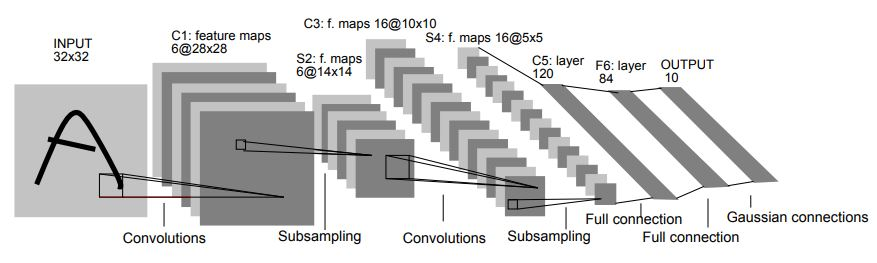
\includegraphics[width=\linewidth, height=5cm, keepaspectratio]{Pictures/convolutional-neural-network/LeNet_Original_Image.jpg}
    \caption{CNN: LeNet}
\end{figure}

\begin{enumerate}
    \item LeNet is a convolutional neural network structure proposed by LeCun et al. in 1998. \cite{ieee/726791/cnn-lenet}
    
    
    \item In general, LeNet refers to LeNet-5 and is a simple convolutional neural network.
\end{enumerate}

\begin{customTableWrapper}{1.3}
\begin{longtable}{|>{\centering\arraybackslash}m{1.5cm}|>{\centering\arraybackslash}m{2cm}|>{\centering\arraybackslash}m{1.5cm}|>{\centering\arraybackslash}c|>{\centering\arraybackslash}m{1cm}|>{\centering\arraybackslash}m{1.5cm}|>{\centering\arraybackslash}m{2cm}|>{\centering\arraybackslash}m{2cm}|}
    \caption{CNN: LeNet-5 Architecture \cite{medium/lenet-5-complete-architecture-84c6d08215f9}}\\

    \hline
    \customTableHeaderColor
    \textbf{Layer No.} & \textbf{Layer} & \textbf{Feature Map} & \textbf{Size} & \textbf{Kernel Size} & \textbf{Stride} & \textbf{Activation} & \textbf{Trainable Params} \\
    \hline
    \endfirsthead

    \hline
    \customTableHeaderColor
    \textbf{Layer No.} & \textbf{Layer} & \textbf{Feature Map} & \textbf{Size} & \textbf{Kernel Size} & \textbf{Stride} & \textbf{Activation} & \textbf{Trainable Params} \\
    \hline
    \endhead

    \hline\endfoot
    \hline\endlastfoot

    Input & Image & 1 & $32\times 32$ & - & - & - & - \\
    \hline

    1 & Convolution & 6 & $28\times 28$ & $5\times 5$ & 1 & tanh & 156 \\
    \hline

    2 & Average Pooling & 6 & $14\times 14$ & $2\times 2$ & 2 & tanh & 0 \\
    \hline

    3 & Convolution & 16 & $10\times 10$ & $5\times 5$ & 1 & tanh & 2416 \\
    \hline

    4 & Average Pooling & 16 & $5\times 5$ & $2\times 2$ & 2 & tanh & 0 \\
    \hline

    5 & Convolution & 120 & $1\times 1$ & $5\times 5$ & 1 & tanh & 48120 \\
    \hline

    6 & FC & - & 84 & - & - & tanh & 10044 \\
    \hline

    Output & FC & - & 10 & - & - & softmax & 850 \\
    \hline
\end{longtable}
\end{customTableWrapper}


\begin{lstlisting}[language=Python,caption=LeNet - tensorflow - Python]
import tensorflow as tf
from tensorflow.keras import layers, models

# Define the model
model = models.Sequential()

# Layer 1: Convolutional Layer
model.add(
    layers.Conv2D(6, (5, 5), 
    activation='tanh', 
    input_shape=(32, 32, 1))
)

# Layer 2: Average Pooling
model.add(layers.AveragePooling2D((2, 2)))

# Layer 3: Convolutional Layer
model.add(layers.Conv2D(16, (5, 5), activation='tanh'))

# Layer 4: Average Pooling
model.add(layers.AveragePooling2D((2, 2)))

# Layer 5: Convolutional Layer
model.add(layers.Conv2D(120, (5, 5), activation='tanh'))

# Flatten the tensor
model.add(layers.Flatten())

# Layer 6: Fully Connected Layer
model.add(layers.Dense(84, activation='tanh'))

# Output Layer: Fully Connected Layer
model.add(layers.Dense(10, activation='softmax'))

# Print the model summary
model.summary()
\end{lstlisting}

\textbf{Output}:
\begin{lstlisting}[numbers=none]
Model: "sequential"
_________________________________________________________________
 Layer (type)                Output Shape              Param #   
=================================================================
 conv2d (Conv2D)             (None, 28, 28, 6)         156
 average_pooling2d (Average  (None, 14, 14, 6)         0
 Pooling2D)
 conv2d_1 (Conv2D)           (None, 10, 10, 16)        2416
 average_pooling2d_1 (Avera  (None, 5, 5, 16)          0
 gePooling2D)
 conv2d_2 (Conv2D)           (None, 1, 1, 120)         48120
 flatten (Flatten)           (None, 120)               0
 dense (Dense)               (None, 84)                10164
 dense_1 (Dense)             (None, 10)                850
=================================================================
Total params: 61706 (241.04 KB)
Trainable params: 61706 (241.04 KB)
Non-trainable params: 0 (0.00 Byte)
_________________________________________________________________
\end{lstlisting}


\section{AlexNet (2012) \cite{gfg-convolutional-neural-network-cnn-in-machine-learning, medium/@siddheshb008/alexnet-architecture-explained-b6240c528bd5,wiki-AlexNet}}\label{cnn: AlexNet}

\begin{figure}[h]
    \centering
    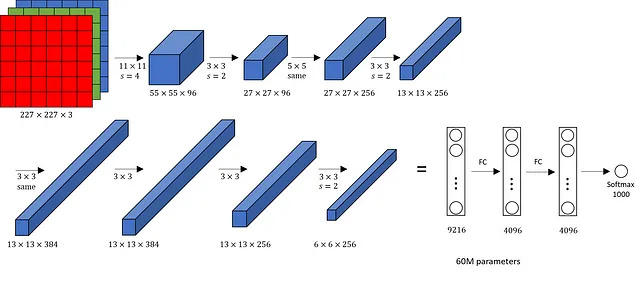
\includegraphics[width=\linewidth, height=5cm, keepaspectratio]{Pictures/convolutional-neural-network/alexnet.jpg}
    \caption{CNN: AlexNet \cite{medium/@siddheshb008/alexnet-architecture-explained-b6240c528bd5}}
\end{figure}

\begin{enumerate}
    \item AlexNet is the name of a convolutional neural network (CNN) architecture, designed by \textbf{Alex Krizhevsky} in collaboration with Ilya Sutskever and Geoffrey Hinton, who was Krizhevsky's Ph.D. advisor at the \textbf{University of Toronto}. \cite{wiki-AlexNet}

    \item This was the first architecture that used GPU to boost the training performance.

    \item Architecture:\\
    \(
      \displaystyle (\text{CNN} \to \text{RN} \to \text{MP})^{2}\to (\text{CNN}^{3} \to \text{MP})\to (\text{FC} \to \text{DO})^{2} \to \text{Linear}\to \text{softmax}  \hfill \text{\cite{wiki-AlexNet}}
    \)

    \begin{customTableWrapper}{1.3}
    \begin{table}[h]
        \centering
        \begin{tabular}{|l l|}
            \hline
            \customTableHeaderColor
            \textbf{Layer} & \textbf{Description} \\ \hline
            CNN & convolutional layer (with ReLU activation) \\
            RN & local response normalization \\
            MP & maxpooling (SEE: \fullref{cnn: Max Pooling}) \\
            FC & fully connected layer (with ReLU activation) \\
            Linear & fully connected layer (without activation) \\
            DO & dropout \\

            \hline
        \end{tabular}
    \end{table}
    \end{customTableWrapper}
\end{enumerate}

\begin{lstlisting}[language=Python,caption=AlexNet - tensorflow - Python]
import tensorflow as tf
from tensorflow.keras import layers, models

model = models.Sequential()

# 1st Convolutional Layer
model.add(layers.Conv2D(96, (11, 11), strides=4, activation='relu', 
        input_shape=(227, 227, 3)))
model.add(layers.MaxPooling2D((3, 3), strides=2))

# 2nd Convolutional Layer
model.add(layers.Conv2D(256, (5, 5), padding='same', activation='relu'))
model.add(layers.MaxPooling2D((3, 3), strides=2))

# 3rd Convolutional Layer
model.add(layers.Conv2D(384, (3, 3), padding='same', activation='relu'))

# 4th Convolutional Layer
model.add(layers.Conv2D(384, (3, 3), padding='same', activation='relu'))

# 5th Convolutional Layer
model.add(layers.Conv2D(256, (3, 3), padding='same', activation='relu'))
model.add(layers.MaxPooling2D((3, 3), strides=2))

# Flatten
model.add(layers.Flatten())

# 1st Fully Connected Layer
model.add(layers.Dense(4096, activation='relu'))
model.add(layers.Dropout(0.5))

# 2nd Fully Connected Layer
model.add(layers.Dense(4096, activation='relu'))
model.add(layers.Dropout(0.5))

# Output Layer
model.add(layers.Dense(1000, activation='softmax'))

# Print the model summary
model.summary()
\end{lstlisting}

\textbf{Output}:

\begin{lstlisting}[numbers=none]
Model: "sequential"
_________________________________________________________________
 Layer (type)                Output Shape              Param #   
=================================================================
 conv2d (Conv2D)             (None, 55, 55, 96)        34944     
 max_pooling2d (MaxPooling2  (None, 27, 27, 96)        0         
 D)                                                              
 conv2d_1 (Conv2D)           (None, 27, 27, 256)       614656    
 max_pooling2d_1 (MaxPoolin  (None, 13, 13, 256)       0         
 g2D)                                                            
 conv2d_2 (Conv2D)           (None, 13, 13, 384)       885120    
 conv2d_3 (Conv2D)           (None, 13, 13, 384)       1327488   
 conv2d_4 (Conv2D)           (None, 13, 13, 256)       884992    
 max_pooling2d_2 (MaxPoolin  (None, 6, 6, 256)         0         
 g2D)                                                            
 flatten (Flatten)           (None, 9216)              0         
 dense (Dense)               (None, 4096)              37752832  
 dropout (Dropout)           (None, 4096)              0         
 dense_1 (Dense)             (None, 4096)              16781312  
 dropout_1 (Dropout)         (None, 4096)              0         
 dense_2 (Dense)             (None, 1000)              4097000   
=================================================================
Total params: 62378344 (237.95 MB)
Trainable params: 62378344 (237.95 MB)
Non-trainable params: 0 (0.00 Byte)
_________________________________________________________________
\end{lstlisting}


\section{VGG-16 (2014) \cite{gfg-convolutional-neural-network-cnn-in-machine-learning,arxiv-1409.1556,gfg-vgg-16-cnn-model}}\label{cnn: VGG-16}

\begin{figure}[h]
    \centering
    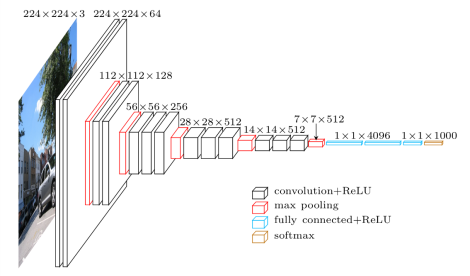
\includegraphics[width=\linewidth, height=7cm, keepaspectratio]{Pictures/convolutional-neural-network/vgg-16-1.png}
    \caption{VGG-16: Architecture - Visual}
\end{figure}
\begin{figure}[h]
    \centering
    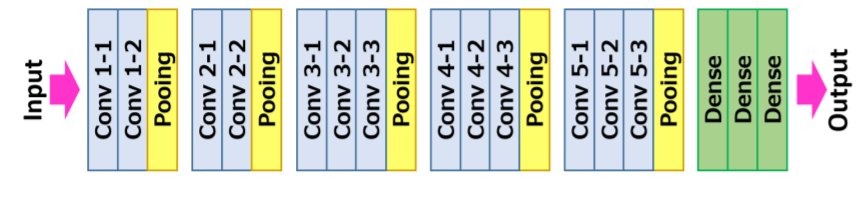
\includegraphics[width=\linewidth, height=2.5cm, keepaspectratio]{Pictures/convolutional-neural-network/vgg-16-2.png}
    \caption{VGG-16: Architecture - Visual (simplified)}
\end{figure}

\begin{enumerate}
    \item The VGG-16 model is a convolutional neural network (CNN) architecture that was proposed by the \textbf{Visual Geometry Group (VGG)} at the \textbf{University of Oxford}.
\end{enumerate}

\begin{lstlisting}[language=Python,caption=VGG-16 - tensorflow - Python]
import tensorflow as tf
from tensorflow.keras import layers, models

model = models.Sequential()

# Block 1
model.add(layers.Conv2D(64, (3, 3), padding='same', activation='relu', 
            input_shape=(224, 224, 3)))
model.add(layers.Conv2D(64, (3, 3), padding='same', activation='relu'))
model.add(layers.MaxPooling2D((2, 2), strides=(2, 2)))

# Block 2
model.add(layers.Conv2D(128, (3, 3), padding='same', activation='relu'))
model.add(layers.Conv2D(128, (3, 3), padding='same', activation='relu'))
model.add(layers.MaxPooling2D((2, 2), strides=(2, 2)))

# Block 3
model.add(layers.Conv2D(256, (3, 3), padding='same', activation='relu'))
model.add(layers.Conv2D(256, (3, 3), padding='same', activation='relu'))
model.add(layers.Conv2D(256, (3, 3), padding='same', activation='relu'))
model.add(layers.MaxPooling2D((2, 2), strides=(2, 2)))

# Block 4
model.add(layers.Conv2D(512, (3, 3), padding='same', activation='relu'))
model.add(layers.Conv2D(512, (3, 3), padding='same', activation='relu'))
model.add(layers.Conv2D(512, (3, 3), padding='same', activation='relu'))
model.add(layers.MaxPooling2D((2, 2), strides=(2, 2)))

# Block 5
model.add(layers.Conv2D(512, (3, 3), padding='same', activation='relu'))
model.add(layers.Conv2D(512, (3, 3), padding='same', activation='relu'))
model.add(layers.Conv2D(512, (3, 3), padding='same', activation='relu'))
model.add(layers.MaxPooling2D((2, 2), strides=(2, 2)))

# Fully connected layers
model.add(layers.Flatten())
model.add(layers.Dense(4096, activation='relu'))
model.add(layers.Dropout(0.5))
model.add(layers.Dense(4096, activation='relu'))
model.add(layers.Dropout(0.5))
model.add(layers.Dense(1000, activation='softmax'))


model.summary()
\end{lstlisting}

\begin{lstlisting}[numbers=none]
Model: "sequential"
_________________________________________________________________
 Layer (type)                Output Shape              Param #   
=================================================================
 conv2d (Conv2D)             (None, 224, 224, 64)      1792      
 conv2d_1 (Conv2D)           (None, 224, 224, 64)      36928     
 max_pooling2d (MaxPooling2  (None, 112, 112, 64)      0         
 D)                                                              
 conv2d_2 (Conv2D)           (None, 112, 112, 128)     73856     
 conv2d_3 (Conv2D)           (None, 112, 112, 128)     147584    
 max_pooling2d_1 (MaxPoolin  (None, 56, 56, 128)       0         
 g2D)                                                            
 conv2d_4 (Conv2D)           (None, 56, 56, 256)       295168    
 conv2d_5 (Conv2D)           (None, 56, 56, 256)       590080    
 conv2d_6 (Conv2D)           (None, 56, 56, 256)       590080    
 max_pooling2d_2 (MaxPoolin  (None, 28, 28, 256)       0         
 g2D)                                                            
 conv2d_7 (Conv2D)           (None, 28, 28, 512)       1180160   
 conv2d_8 (Conv2D)           (None, 28, 28, 512)       2359808   
 conv2d_9 (Conv2D)           (None, 28, 28, 512)       2359808   
 max_pooling2d_3 (MaxPoolin  (None, 14, 14, 512)       0         
 g2D)                                                            
 conv2d_10 (Conv2D)          (None, 14, 14, 512)       2359808   
 conv2d_11 (Conv2D)          (None, 14, 14, 512)       2359808   
 conv2d_12 (Conv2D)          (None, 14, 14, 512)       2359808   
 max_pooling2d_4 (MaxPoolin  (None, 7, 7, 512)         0         
 g2D)
 flatten (Flatten)           (None, 25088)             0         
 dense (Dense)               (None, 4096)              102764544 
 dropout (Dropout)           (None, 4096)              0         
 dense_1 (Dense)             (None, 4096)              16781312  
 dropout_1 (Dropout)         (None, 4096)              0         
 dense_2 (Dense)             (None, 1000)              4097000   
=================================================================
Total params: 138357544 (527.79 MB)
Trainable params: 138357544 (527.79 MB)
Non-trainable params: 0 (0.00 Byte)
_________________________________________________________________
\end{lstlisting}


\section{Region Based CNNs (R-CNN/ RCNN) (2013) \cite{arxiv-1311.2524v5-rcnn,https://www.geeksforgeeks.org/r-cnn-region-based-cnns/}}\label{Region Based CNNs (R-CNN/ RCNN)}

\begin{figure}[H]
    \centering
    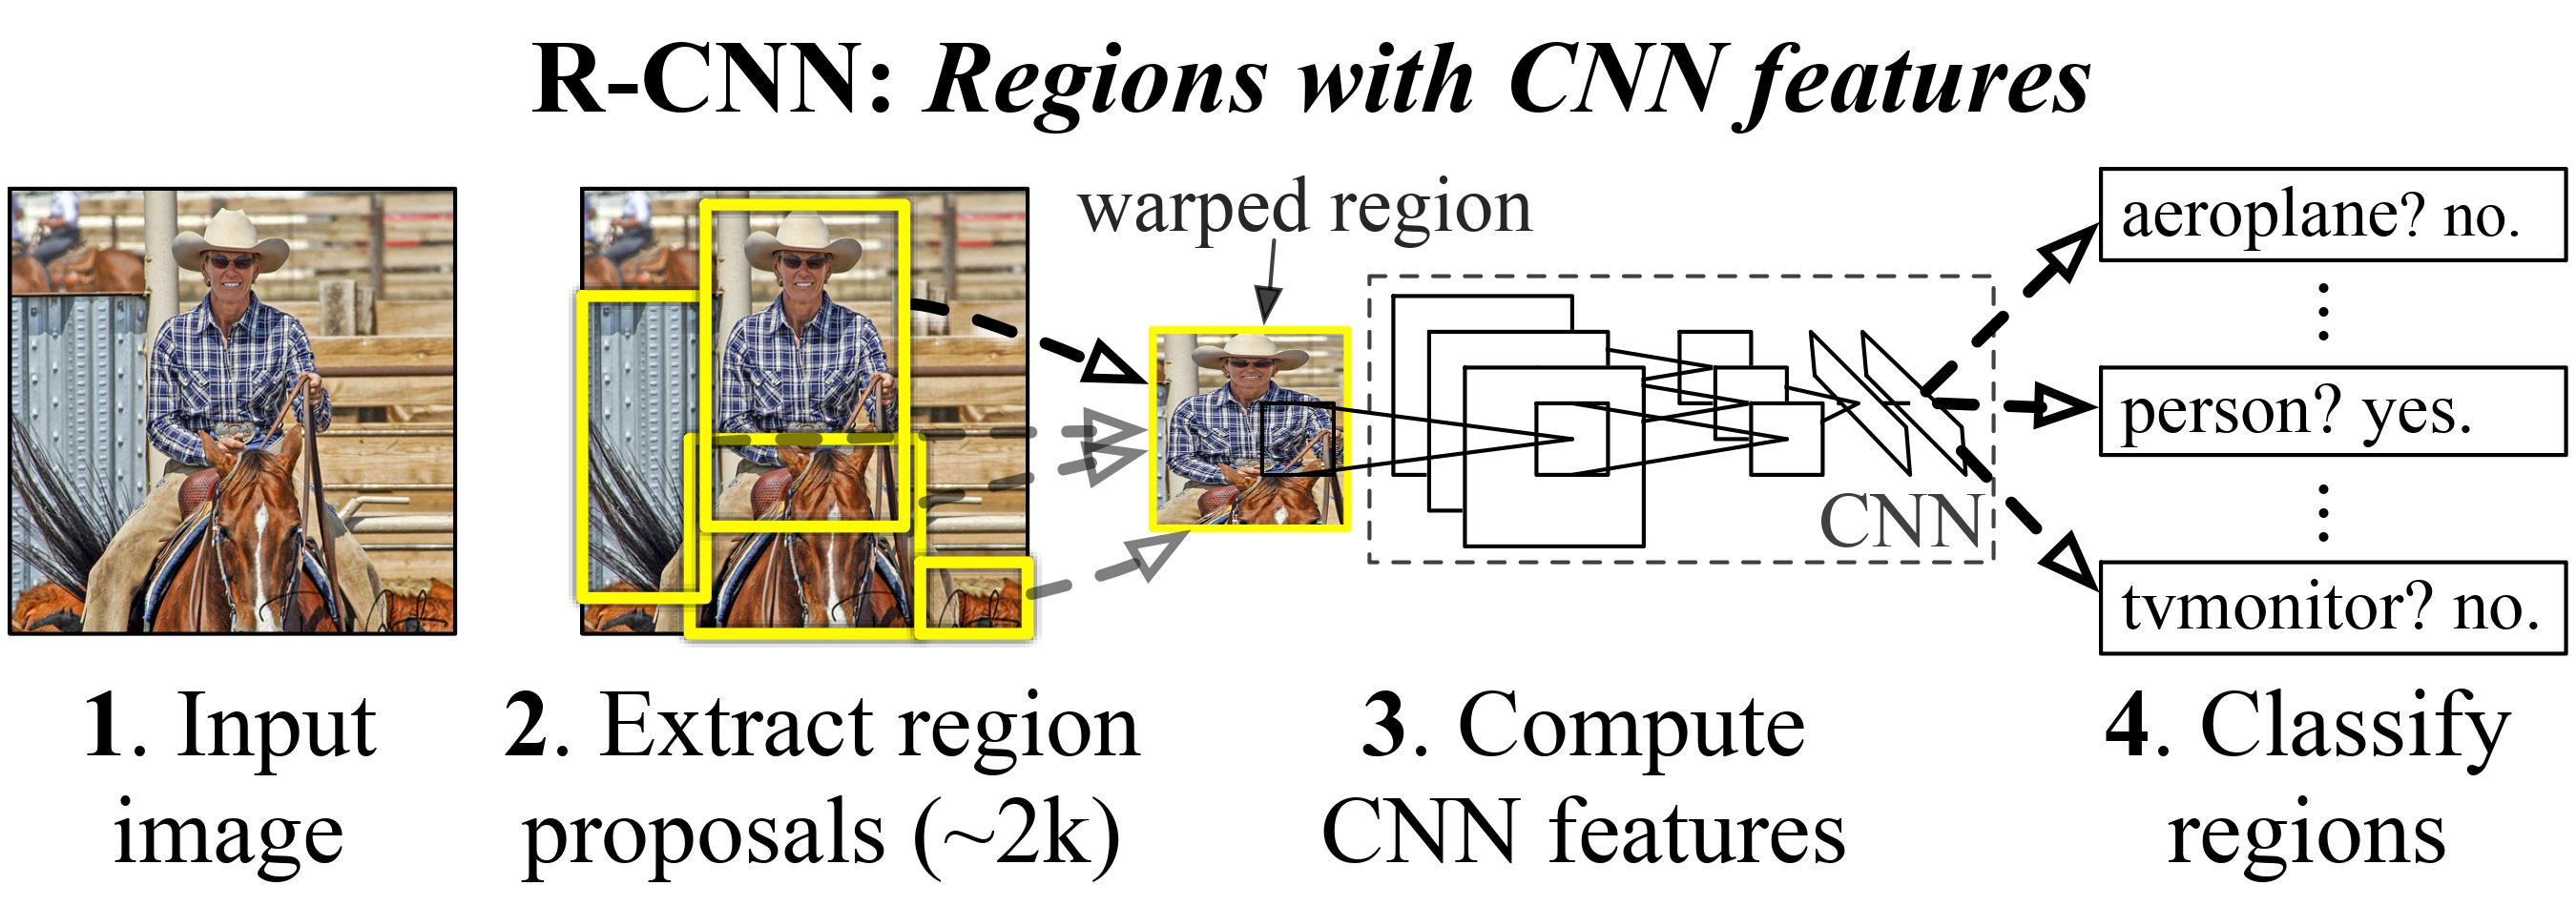
\includegraphics[width=\linewidth, height=3.5cm, keepaspectratio]{Pictures/convolutional-neural-network/rcnn-splash-method.jpg}
    \caption{R-CNN}
\end{figure}

\begin{enumerate}
    \item Convolution Neural Network (CNN) with a fully connected layer is \textbf{NOT} able to deal with the frequency of occurrence and multi objects.

    \item We can use a sliding window brute force search to select a region and apply the CNN model to that.\\
    \textbf{Disadvantages}:
    \begin{enumerate}
        \item same object can be represented in an image with different sizes and different aspect ratios.

        \item we will have a lot of region proposals and if we apply deep learning (CNN) to all those regions that would computationally very expensive.

    \end{enumerate}
    
\end{enumerate}

\subsection{Region Proposals \cite{arxiv-1311.2524v5-rcnn,https://www.geeksforgeeks.org/r-cnn-region-based-cnns/}}

\begin{table}[H]
    \begin{minipage}[t]{0.49\linewidth}
        \begin{figure}[H]
            \centering
            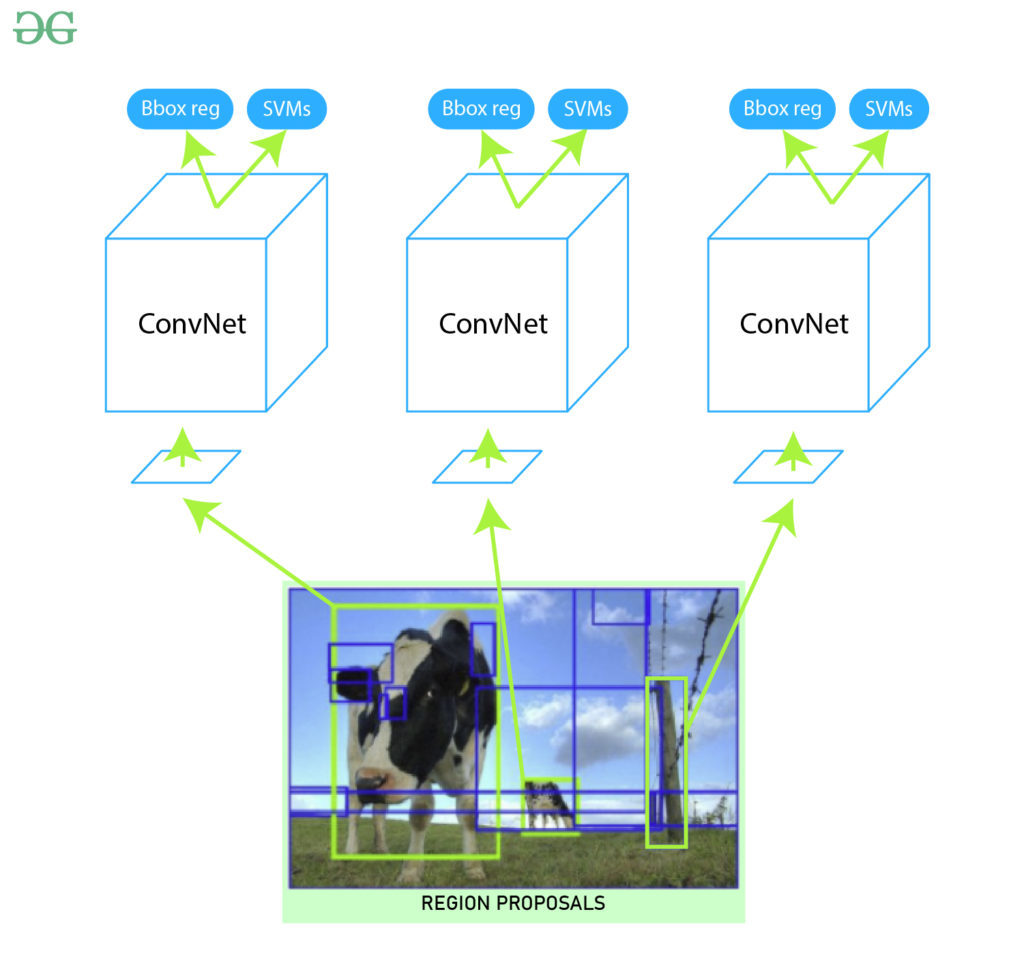
\includegraphics[width=\linewidth, height=3cm, keepaspectratio]{Pictures/convolutional-neural-network/rcnn-region-proposals.jpg}
            \caption{RCNN: Region Proposals}
        \end{figure}        
    \end{minipage}
    \hfill
    \begin{minipage}[t]{0.49\linewidth}
        \begin{enumerate}
            \item Region proposals are simply the smaller regions of the image that possibly contains the objects we are searching for in the input image.
        
            \item To reduce the region proposals in the R-CNN uses a greedy algorithm called \textbf{selective search} (SEE: \fullref{Selective Search (CNN)}).
        \end{enumerate}
    \end{minipage}
\end{table}


\subsection{Bounding Box Regressor (BB-regression) \cite{https://www.geeksforgeeks.org/r-cnn-region-based-cnns/}}\label{Bounding Box Regressor (BB-regression)}

\begin{enumerate}
    \item In order to precisely locate the bounding box in the image, we used a scale-invariant linear regression model called \textbf{bounding box regressor}.

    \item For training this model we take as predicted and Ground truth pairs of four dimensions of localization.\\
    These dimensions are $(x, y, w, h)$ where:
    \begin{enumerate}
        \item $x$ and $y$ are the pixel coordinates of the center of the bounding box respectively. 

        \item $w$ and $h$ represent the width and height of bounding boxes.
    \end{enumerate}
    
    \item This method increases the \textbf{Mean Average precision (mAP)} of the result by $3-4\%$.
    
\end{enumerate}



\subsection*{Output}
\begin{enumerate}
    \item Now we have region proposals that are classified for every class label. 
    
    \item In order to deal with the extra bounding box generated by the above model in the image, we use an algorithm called \textbf{Non-maximum suppression} (SEE: \fullref{Non-maximum Suppression (NMS)}).\\
    It works in 3 steps:
    \begin{enumerate}
        \item Discard those objects where the confidence score is less than a certain threshold value(say $0.5$).

        \item Select the region which has the highest probability among candidates regions for the object as the predicted region.

        \item In the final step, we discard those regions which have \textbf{IoU (intersection Over Union)} (SEE: \fullref{IOU (Intersection over Union)}) with the predicted region over $0.5$.

    \end{enumerate}
\end{enumerate}

\subsection*{Challenges}
\begin{enumerate}
    \item Since there are approximately 2000 candidate proposals. It takes a lot of time to train the network. Also, we need to train multiple steps separately (CNN architecture, SVM model, bounding box regressor). So, This makes it very slow to implement.

    \item \textbf{R-CNN} (SEE: \fullref{Region Based CNNs (R-CNN/ RCNN)}) cannot be used in real-time because it takes approximately 50 sec to test an image with a bounding box regressor.

    \item Since we need to save feature maps of all the region proposals. It also increases the amount of disk memory required during training.
\end{enumerate}


\section{Fast R-CNN (2015) \cite{arxiv/1504.08083-fast-rcnn,medium/towardsdatascience.com/fast-r-cnn-for-object-detection-a-technical-summary-a0ff94faa022}}\label{Fast R-CNN}

\begin{figure}[h]
    \centering
    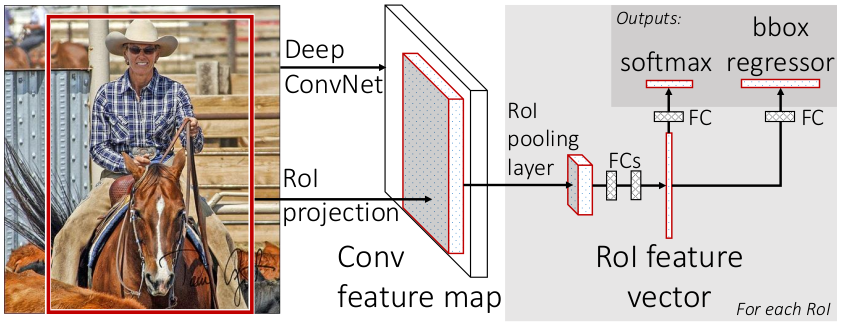
\includegraphics[width=\linewidth, height=3cm, keepaspectratio]{Pictures/convolutional-neural-network/fast-rcnn-arch.png}
    \caption{Fast-RCNN: Architecture \cite{arxiv/1504.08083-fast-rcnn}}
\end{figure}

\begin{enumerate}
    \item The Fast R-CNN consists of a CNN (usually pre-trained on the ImageNet classification task) with its final pooling layer replaced by an “ROI pooling” layer and its final FC layer is replaced by two branches - a $(K + 1)$ category \textbf{softmax layer}(SEE: \fullref{Softmax function}) branch and a category-specific bounding box regression branch.

    \item The entire image is fed into the backbone CNN and the features from the last convolution layer are obtained. Depending on the backbone CNN used, the output feature maps are much smaller than the original image size. This depends on the stride of the backbone CNN, which is usually 16 in the case of a VGG backbone.

    \item The \textbf{object proposal windows} are obtained from a region proposal algorithm like \textbf{selective search} (SEE: \fullref{Selective Search (CNN)}). As explained in Regions with CNNs, object proposals are rectangular regions on the image that signify the presence of an object.

    \item The portion of the backbone feature map that belongs to this window is then fed into the \textbf{ROI Pooling layer} (SEE: \fullref{cnn: Region of Interest (ROI) Pooling Layer}).

    \item The output features from the ROI Pooling layer are then fed into the successive FC layers, and the softmax and BB-regression (SEE: \fullref{Bounding Box Regressor (BB-regression)}) branches. The softmax classification branch produces probability values of each ROI belonging to $K$ categories and one catch-all background category. The BB regression branch output is used to make the bounding boxes from the region proposal algorithm more precise.
\end{enumerate}

\subsection*{Loss}
\[
    \displaystyle
    L_{loc}(t^u, v) = \sum_{i \in \dCurlyBrac{x,y,w,h}} \operatorname{smooth}_{L_1}(t_i^u - v_i)
    \hfill
    \text{(For BB-Regression)}
\]
\[
    \displaystyle
    L(p,u,t^u,v) = L_{cls}(p,u) + \lambda[u\geq 1]L_{loc}(t^u, v)
    \hfill
    (\text{Multi-task loss})
\]

\noindent \textbf{Where},
\begin{customTableWrapper}{1.3}
\begin{table}[h]
    \begin{tabular}{l l}
        $K+1$ & Number of categories \\ \hline

        $p_i$ & Category ($i=0,\cdots,K$) \\
        $u$ & true class ($0/1$) \\ \hline

        $v$ & ground truth bounding box \\
        $t^u = (t^u_x,t^u_y,t^u_w,t^u_h)$ & predicted bounding box \\ \hline

        $L_{cls}(p,u) = -\log(p_u)$ & Classification loss \\
        $L_{loc}(t^u,v)$ & localization loss \\
    \end{tabular}
\end{table}
\end{customTableWrapper}


\section{Faster R-CNN (2015) \cite{arxiv/1506.01497-faster-rcnn,gfg/faster-r-cnn-ml}}\label{Faster R-CNN}

\url{https://www.geeksforgeeks.org/faster-r-cnn-ml/}\\
\url{https://arxiv.org/abs/1506.01497}


\section{Network In Network (NiN) \cite{arxiv/1312.4400-nin,medium/towardsdatascience.com/review-nin-network-in-network-image-classification-69e271e499ee}}\label{Network In Network (NiN)}

TODO













































































































































